\documentclass[tikz,border=2pt]{standalone}
\usepackage{amsmath,amssymb}
\usepackage{tikz}
\usetikzlibrary{arrows.meta}

\begin{document}
% The graphical method in four steps: draw the constraint boundaries, shade the feasible
% region, draw one objective line, slide it in the improving direction until it is about to
% leave the region.
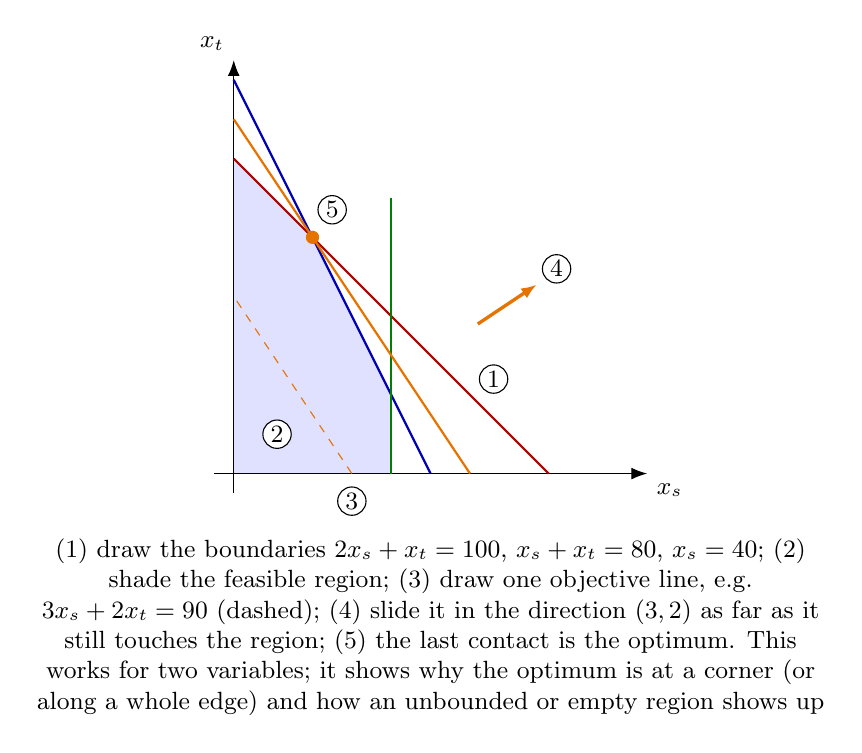
\begin{tikzpicture}[x=0.05cm, y=0.05cm, every node/.style={font=\small}, >={Latex[length=2mm]}, num/.style={font=\small, circle, draw, inner sep=1pt, fill=white}]
	\fill[blue!12] (0,0) -- (40,0) -- (40,20) -- (20,60) -- (0,80) -- cycle;
	\draw[->] (-5,0) -- (105,0) node[below right] {$x_s$};
	\draw[->] (0,-5) -- (0,105) node[above left] {$x_t$};
	\draw[blue!70!black, thick] (50,0) -- (0,100);
	\draw[red!70!black, thick] (80,0) -- (0,80);
	\draw[green!50!black, thick] (40,0) -- (40,70);
	\draw[orange!90!black, dashed] (30,0) -- (0,45);
	\draw[->, orange!90!black, very thick] (62,38) -- (77,48);
	\draw[orange!90!black, thick] (60,0) -- (0,90);
	\fill[orange!90!black] (20,60) circle (2.4pt);
	\node[num] at (66,24) {1};
	\node[num] at (11,10) {2};
	\node[num] at (30,-7) {3};
	\node[num] at (82,52) {4};
	\node[num] at (25,67) {5};
	\node[anchor=north, align=flush center, text width=10cm] at (50,-14) {(1) draw the boundaries $2x_s+x_t=100$, $x_s+x_t=80$, $x_s=40$; (2) shade the feasible region; (3) draw one objective line, e.g. $3x_s+2x_t=90$ (dashed); (4) slide it in the direction $(3,2)$ as far as it still touches the region; (5) the last contact is the optimum. This works for two variables; it shows why the optimum is at a corner (or along a whole edge) and how an unbounded or empty region shows up};
\end{tikzpicture}
\end{document}
